%-------------------------------------------------------------------------------
\tikzset{fl/.style={ draw, fill = gray,rectangle,minimum size=3mm}}
\tikzset{sub/.style={ draw, shape border rotate=90, isosceles triangle,minimum size=8mm,yshift=-8mm}}
%-------------------------------------------------------------------------------
%-------------------------------------------------------------------------------
\chapter{Tableaux persistants}
%-------------------------------------------------------------------------------
%-------------------------------------------------------------------------------
\thispagestyle{empty}
%-------------------------------------------------------------------------------
%-------------------------------------------------------------------------------
\begin{abstract}
La notion de tableaux est centrale dans les langages informatiques. Le type usuel est une structure impérative : les changements ne créent pas un nouveau tableau mais modifient le tableau "en place". Nous allons définir le type de données tableau et en construire une implémentation persistante.
\end{abstract}


%-------------------------------------------------------------------------------
%-------------------------------------------------------------------------------
%-------------------------------------------------------------------------------
\section{Définition}
%-------------------------------------------------------------------------------
%-------------------------------------------------------------------------------
%-------------------------------------------------------------------------------
 On peut voir un tableau comme une fonction depuis un ensemble fini $\{0, 1, \ldots, n-1\}$ vers l'ensemble des valeurs du type choisi.  Cependant, pour des raisons de simplicité nous allons définir des tableaux de taille $n$ dont les indices décrivent $\{1, 2, \ldots, n\}$.
 
 Voici les principales fonctions définies pour le type \type{Array} :

\begin{enumerate}
\item \type{Array.make n x} crée un tableau de taille $n$ dont les éléments sont tous $x$.
\begin{lstlisting}
Array.make : int -> 'a -> 'a array
\end{lstlisting}

\item \type{Array.length t} renvoie la longueur du tableau $t$
\begin{lstlisting}
Array.length : 'a array -> int
\end{lstlisting}

\item \type{Array.get k t} renvoie l'élément d'indice $k$ du tableau $t$, c'est l'équivalent de \type{t.(k)}
\begin{lstlisting}
Array.get : int -> 'a array -> 'a
\end{lstlisting}

\item \type{Array.set k t y} met la valeur $y$ à la position $k$ dans le tableau $t$, c'est \type{t.(k) <- x}
\begin{lstlisting}
Array.set : int -> 'a array -> 'a -> unit
\end{lstlisting}
\end{enumerate}

\medskip

Il y en a d'autres, moins utilisés.

Nous allons nous intéresser à l'initialisation par une fonction :
\type{Array.init n f} renvoie le tableau de taille $n$ dont les éléments sont tels que la valeur en $i$ soit $f(i)$

\begin{lstlisting}
Array.init : int -> (int -> 'a) -> 'a array
\end{lstlisting}

et à l'extraction d'une tranche  : 
\type{Array.sub t i p} renvoie le tableau de taille $p$ dont les éléments sont ceux de $t$, dans le même ordre, d'indice $i$, $i+1$ \dots $i+p-1$.

C'est l'équivalent de \Type{t[i, i+p]} dans python.
\begin{lstlisting}
Array.sub : 'a array -> int -> int -> 'a array
\end{lstlisting}


Le caractère impératif du type se voit uniquement dans la la fonction \type{set} : celle-ci ne renvoie rien\footnote{En fait, elle renvoie \type{()}, la valeur du type \type{unit}.}

\newpage

Nous allons définir un type de données persistant, \Type{tableau}, avec les mêmes fonctions (dont on change le nom) : 
\begin{enumerate}
\item \type{creer n x} crée un tableau de taille $n$ dont les éléments sont tous $x$.
\begin{lstlisting}
creer : int -> 'a -> 'a tableau
\end{lstlisting}

\item \type{longueur t} renvoie la longueur du tableau $t$
\begin{lstlisting}
longueur : 'a tableau -> int
\end{lstlisting}

\item \type{valeur k t} renvoie l'élément d'indice $k$ du tableau $t$
\begin{lstlisting}
valeur : int -> 'a tableau -> 'a
\end{lstlisting}

\item \type{changer k t y} met la valeur $y$ à la position $k$ dans le tableau $t$ en renvoyant un nouveau tableau, modifié et laissant inchangé le tableau initial.
\begin{lstlisting}
changer : int -> 'a tableau -> 'a -> 'a tableau
\end{lstlisting}

\item \type{construire n f} renvoie le tableau des $f(1)$, $f(2)$, \ldots, $f(n)$
\begin{lstlisting}
construire : int -> (int -> 'a) -> 'a tableau
\end{lstlisting}

\item L'extraction est trop difficile à écrire, on se contentera de

\type{debut t  p} qui renvoie le tableau des $p$ élément initiaux de $t$
\begin{lstlisting}
debut : 'a tableau -> int ->  'a tableau
\end{lstlisting}
\end{enumerate}

Bien entendu, on souhaite que les opérations se fassent rapidement, un temps constant est généralement difficile à obtenir pour des structures persistantes mais une complexité logarithmique est espérée.

Cela interdit de recopier un tableau classique quand on change un des éléments.
%-------------------------------------------------------------------------------
%-------------------------------------------------------------------------------
%-------------------------------------------------------------------------------
\section{Choix de l'implémentation}
%-------------------------------------------------------------------------------
%-------------------------------------------------------------------------------
%-------------------------------------------------------------------------------
Une complexité logarithmique est possible avec un arbre à condition de savoir comment descendre les branches. On propose la stratégie suivante pour rechercher le nœud d'indice $k$ :

\begin{itemize}
    \item si $k=1$ on a trouvé, l'élément est à la racine,
    \item si $k>1$ avec $k$ pair, on cherche \type{k/2} dans le fils gauche,
    \item si $k>1$ avec $k$ impair, on cherche \type{k/2} dans le fils droit.
\end{itemize}

Par exemple, l'élément d'indice 37 sera trouvé 
\begin{itemize}
    \item en cherchant 18 dans le fils droit
    \item puis en cherchant 9 dans le petit fils gauche
    \item puis 4 à droite
    \item puis 2 à gauche
    \item la valeur est la racine du fils gauche.
\end{itemize}

Dans le dessin suivant on a donné les positions d'un tableau à 37 éléments.

\begin{center}
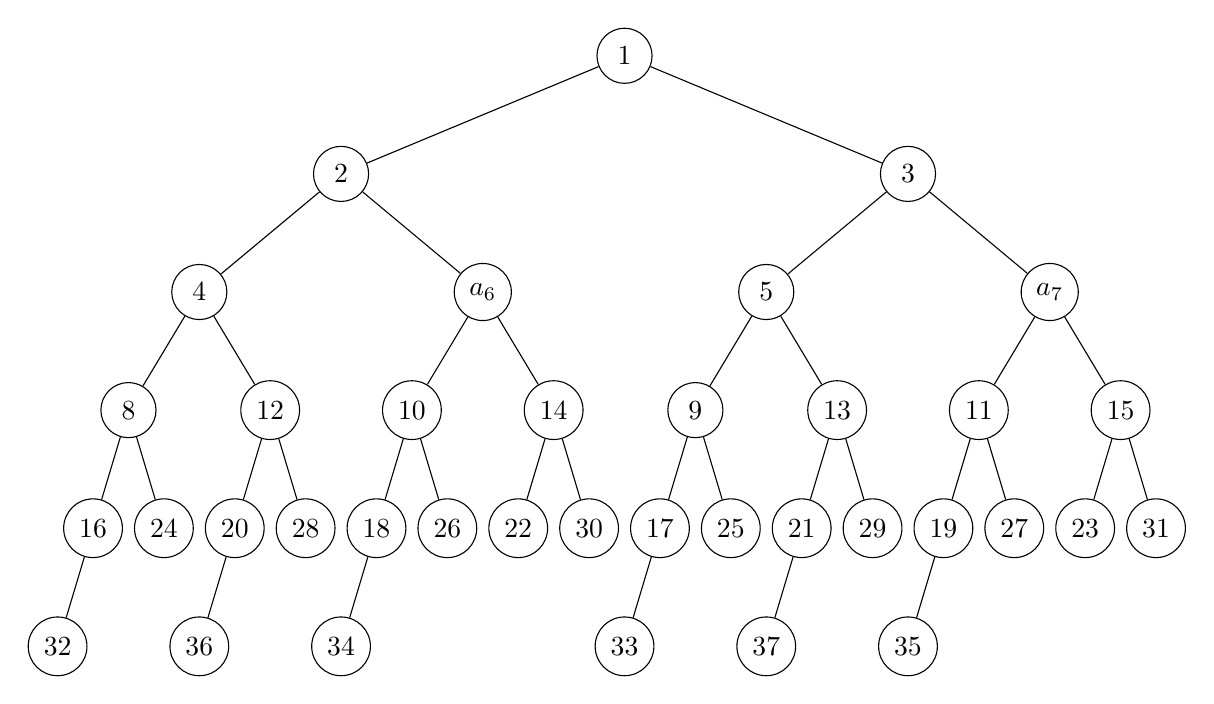
\begin{tikzpicture}[level distance =15mm,minimum size =7mm]
  \tikzstyle{level 1}=[sibling distance =72mm]
  \tikzstyle{level 2}=[sibling distance =36mm]
  \tikzstyle{level 3}=[sibling distance =18mm]
  \tikzstyle{level 4}=[sibling distance =9mm]
  \tikzstyle{every node}=[circle,draw]
  \node {$1$}
   child {node {$2$}
          child {node {$4$}
                 child {node {$8$}
                        child {node {16}
                               child {node{32}}
                               child {edge from parent[draw=none]}
                              }
                        child {node {24}}
                       }
                 child {node {$12$}
                        child {node {20}
                               child {node{36}}
                               child {edge from parent[draw=none]}
                              }
                        child {node {28}}
                       }
                }
          child {node {$a_6$}
                 child {node {$10$}
                        child {node {18}
                               child {node{34}}
                               child {edge from parent[draw=none]}
                              }
                        child {node {26}}
                       }
                 child {node {$14$}
                        child {node {22}}
                        child {node {30}}
                       }
                }
        }
   child {node {$3$}
          child {node {$5$}
                 child {node {$9$}
                        child {node {17}
                               child {node{33}}
                               child {edge from parent[draw=none]}
                              }
                        child {node {25}}
                       }
                 child {node {$13$}
                        child {node {21}
                               child {node{37}}
                               child {edge from parent[draw=none]}
                              }
                        child {node {29}}
                       }
                }
          child {node {$a_7$}
                 child {node {$11$}
                        child {node {19}
                               child {node{35}}
                               child {edge from parent[draw=none]}
                              }
                        child {node {27}}
                       }
                 child {node {$15$}
                        child {node {23}}
                        child {node {31}}
                       }
                }
        };
\end{tikzpicture}
\end{center}

On va donc utiliser un arbre binaire qui sera accompagné de la taille pour que celle-ci soit directement calculable (et le contrôle des indices facile aussi).

\begin{lstlisting}
type 'a arbre = Vide | Noeud of 'a arbre * 'a * 'a arbre;;
type 'a tableau = {taille : int;
                   data : 'a arbre};;
\end{lstlisting}
%-------------------------------------------------------------------------------
%-------------------------------------------------------------------------------
%-------------------------------------------------------------------------------
\section{Les fonctions}
%-------------------------------------------------------------------------------
%-------------------------------------------------------------------------------
%-------------------------------------------------------------------------------
\subsection{Premières fonctions}
%-------------------------------------------------------------------------------
%-------------------------------------------------------------------------------
\begin{Exercise}[title = Taille]\it 
Écrire la fonction \type{longueur}.
\end{Exercise}
%-------------------------------------------------------------------------------
\begin{Answer}
\begin{lstlisting}
let longueur t = t.taille;;
\end{lstlisting}
\end{Answer}
%-------------------------------------------------------------------------------
%-------------------------------------------------------------------------------
\begin{Exercise}[title = Accès]\it 
Écrire la fonction \type{valeur}.
\end{Exercise}
%-------------------------------------------------------------------------------
\begin{Answer}
\begin{lstlisting}
let valeur k t =
  let rec lire p a =
    match a, p with
      |Vide, _ -> failwith "Indice trop grand"
      |_, p when p < 1 -> failwith "Indice trop petit"
      |Noeud(g, r, d), 1 -> r
      |Noeud(g, r, d), p when p mod 2 = 0 -> lire (p/2) g
      |Noeud(g, r, d), p -> lire (p/2) d in
    lire k t.data;;
\end{lstlisting}
\end{Answer}
%-------------------------------------------------------------------------------
%-------------------------------------------------------------------------------
\begin{Exercise}[title = Modification]\it 
Écrire la fonction \type{changer}.
\end{Exercise}
%-------------------------------------------------------------------------------
\begin{Answer}
\begin{lstlisting}
let changer k t x =
  let rec ecrire p a =
    match a, p with
      |Vide, _ -> failwith "Indice trop grand"
      |_, p when p < 1 -> failwith "Indice trop petit"
      |Noeud(g, r, d), 1 -> Noeud(g, x, d)
      |Noeud(g, r, d), p when p mod 2 = 0 
                         -> Noeud(ecrire (p/2) g, r, d) 
      |Noeud(g, r, d), p -> Noeud(g, r, ecrire (p/2) d )in
    {taille = t.taille; data = ecrire k t.data};;
\end{lstlisting}
\end{Answer}
%-------------------------------------------------------------------------------
%-------------------------------------------------------------------------------
\begin{Exercise}[title = Complexité]\it 
Quelle est la hauteur de l'arbre associée à un tableau de taille $n$ ?

En déduire la complexité des fonctions ci-dessus.
\end{Exercise}
%-------------------------------------------------------------------------------
\begin{Answer}
La profondeur du nœud associé à 1 est 0. Si on note $p(k)$ la profondeur du nœud associé à $k$ on a $p(k) = 1 + p(k/2)$. On en déduit par récurrence sur $m$ que, pour $2^m \le k < 2^{m+1}$, $p(k) = m$. Ainsi la hauteur est $\left\lfloor \log_2(n)\right\rfloor$.

La complexité de \type{taille} est constante et \type{valeur} et \type{changer} sont donc de complexité logarithmique. 
\end{Answer}
%-------------------------------------------------------------------------------
%-------------------------------------------------------------------------------
\subsection{Constructions}
%-------------------------------------------------------------------------------
%-------------------------------------------------------------------------------
\begin{Exercise}[title = Nombres d'éléments]\it 
Prouver que l'arbre associée à un tableau est quasi-complet.

Combien y-a-t-il d'éléments dans les fils droits et gauches de l'arbre associée à un tableau de taille $n$ ?.
\end{Exercise}
%-------------------------------------------------------------------------------
\begin{Answer}
Pour $2^m \le n < 2^{m+1}$, les entiers $k$ tels que $2^h \le k < 2^{h+1}$ remplissent le niveau de profondeur $h$ pour $h< m$. 

Pour $n$ impair, $n = 2m+1$, il y a $m$ termes pairs et $m$ impairs entre 2 et $n$, et pour $n$ pair, $n = 2m$, il y a $m$ termes pairs et $m-1$ impairs entre 2 et $n$. Il y a donc \type{m/2} éléments dans le fils gauche et \type{(m-1) /2} éléments dans le fils droit.
\end{Answer}
%-------------------------------------------------------------------------------
%-------------------------------------------------------------------------------
\begin{Exercise}[title = Création]\it 
Écrire la fonction \type{creer}.
\end{Exercise}
%-------------------------------------------------------------------------------
\begin{Answer}
\begin{lstlisting}
let creer n x =
  let rec aux k =
    match k with
      |0 -> Vide
      |_ -> Noeud(aux (k/2), x, aux (k-1)/2) in
    if n < 1
    then failwith "La longueur doit être strictement positive"
    else {taille = n; data = aux n};;
\end{lstlisting}
\newpage
\end{Answer}
%-------------------------------------------------------------------------------
%-------------------------------------------------------------------------------
\begin{Exercise}[title = Initialisation]\it 
Écrire la fonction \type{construire}.

On essaiera d'écrire une fonction de complexité linéaire et non en ${\cal O}\bigl(n\log(n)\bigr)$.
\end{Exercise}
%-------------------------------------------------------------------------------
\begin{Answer}
\begin{lstlisting}
let construire n f =
  let rec aux n f =
    match n with
      |0 -> Vide
      |_ -> let g = aux (n/2) (fun k -> f (2*k)) in
          let d = aux ((n-1)/2) (fun k -> f (2*k+1)) in
            Noeud(g, f 1, d) in
    if n < 1
    then failwith "La longueur doit être strictement positive"
    else {taille = n; data = aux n f};;
\end{lstlisting}
\end{Answer}
%-------------------------------------------------------------------------------
%-------------------------------------------------------------------------------
\begin{Exercise}[title = Extraction]\it 
Écrire la fonction \type{debut}.
\end{Exercise}
%-------------------------------------------------------------------------------
\begin{Answer}
\begin{lstlisting}
let debut t  p = 
  if p > t.taille
  then failwith "Il n'y a pas assez d'éléments"
  else let rec extr ar k =
         match ar, k with 
           |Vide, _ -> Vide
           |_, 0 -> Vide
           |Noeud(g, r, d), k -> 
               Noeud(extr g (k/2), r, extr d ((k-1)/2)) in 
      {taille = p; data = extr t.data p};;
\end{lstlisting}
\end{Answer}
%-------------------------------------------------------------------------------
%-------------------------------------------------------------------------------
\subsection{Nouvelles fonctions}
%-------------------------------------------------------------------------------
%-------------------------------------------------------------------------------
Un avantage de cette implémentation est qu'elle permet de travailler dynamiquement : on peut ajouter un élément à la fin du tableau ou enlever le dernier élément.

Dans les questions $n$ est la longueur des tableaux.
%-------------------------------------------------------------------------------
%-------------------------------------------------------------------------------
\begin{Exercise}[title = Ajouter]\it 
Écrire une fonction \type{plus t x} qui ajoute l'élément $x$ dans un nouveau tableau reprenant les éléments de $t$.
\end{Exercise}
%-------------------------------------------------------------------------------
\begin{Answer}
\begin{lstlisting}
let plus t x =
  let rec add p a =
    match a, p with
      |_, 1 -> Noeud(Vide, x, Vide)
      |Vide, _ -> failwith "Ceci ne devrait pas arriver"
      |Noeud(g, r, d), p when p mod 2 = 0 -> Noeud(add (p/2) g, r, d) 
      |Noeud(g, r, d), p -> Noeud(g, r, add (p/2) d )
  and n  = t.taille +1 in
    {taille = n; data = add n t.data};;
\end{lstlisting}
\end{Answer}
%-------------------------------------------------------------------------------
%-------------------------------------------------------------------------------
\begin{Exercise}[title = Enlever]\it 
Écrire une fonction \type{moins t} qui renvoie un couple formé du tableau des $n-1$ premiers éléments de \type{t} et du dernier élément.
\end{Exercise}
%-------------------------------------------------------------------------------
\begin{Answer}
\begin{lstlisting}
let moins t =
  let rec del p a =
    match a, p with
      |Noeud(g, r, d), 1 -> Vide, r
      |Vide, _ -> failwith "Ceci ne devrait pas arriver"
      |Noeud(g, r, d), p when p mod 2 = 0 -> 
          let g1, x = del (p/2) g in Noeud(g1, r, d), x
      |Noeud(g, r, d), p -> 
          let d1, x = del (p/2) d in Noeud(g, r, d1), x
  and n  = t.taille in
  let a, x = del n t.data in {taille = n-1; data = a}, x;;
\end{lstlisting}
\newpage
\end{Answer}
%-------------------------------------------------------------------------------
%-------------------------------------------------------------------------------
\medskip

Il est souvent utile d'écrire les fonctions de conversion.
%-------------------------------------------------------------------------------
%-------------------------------------------------------------------------------
\begin{Exercise}[title = Tableau vers array]\it 
Écrire une fonction \type{vers\_array t} qui reçoit un tableau et renvoie l'objet de type \type{array} dont les éléments d'indices 0 à $n-1$ sont ceux d'indices 1 à $n$ du tableau.
\end{Exercise}
%-------------------------------------------------------------------------------
\begin{Answer}
\begin{lstlisting}
let vers_array t =
  let n = t.taille in
  let rec aux ar k =
    match ar with
      |Vide -> [||]
      |Noeud(g, r, d) -> 
          let ag = aux g (k/2)
          and ad = aux d ((k-1)/2) 
          and a = Array.make n r in
            for i = 0 to (k-2) do
              if i mod 2 = 0
              then a.(i+1) <- ag.(i/2)
              else a.(i+1) <- ad.(i/2) done;
            a
  in aux t.data n;;
\end{lstlisting}
\end{Answer}
%-------------------------------------------------------------------------------
%-------------------------------------------------------------------------------
\begin{Exercise}[title = Array vers tableau]\it 
Écrire une fonction \type{vers\_tableau t} qui reçoit objet de type \type{array} et renvoie le tableau dont les éléments d'indices 1 à $n$ sont ceux d'indices 1 à $n$ de $t$.
\end{Exercise}
%-------------------------------------------------------------------------------
\begin{Answer}
\begin{lstlisting}
let vers_tableau t =
  let f k = t.(k-1) 
  and n = Array.length t in
    construire n f;;
\end{lstlisting}
\end{Answer}
%-------------------------------------------------------------------------------
%-------------------------------------------------------------------------------

